\pagebreak %I will take those out later, for now they will help me to write

\section{Baumslag-Solitar groups and their generalisation}

In this chapter we will explore a certain class of groups, which were initially introduced in \cite{BaSo62}. They have since served as examples and counterexamples of groups with different properties.

\subsection{Definition and first properties}

\begin{definition}
    A \emph{Baumslag-Solitar group $BS(m,n)$} is a group given by the presentation \[BS(m,n) = \langle \: a, t\:|\:t(a^m)t^{-1} = a^n \: \rangle \] where $m,n \in \Z \setminus \{0\}$.
\end{definition}

\begin{remark}
    Note, that for $m = n = 1$, $BS(m,n) = \langle a,t \: | \: tat^{-1} = a \: \rangle \cong \Z \times \Z$. This case seems to be regarded as somehow seperate in the literature.
\end{remark}

The first property of these groups that we will consider, and the one that motivated Baumslag and Solitar in \cite{BaSo62}, is that of being (non-)Hopfian.

\begin{definition}
    A group $G$ is said to be \emph{Hopfian} if every epimorphism from $G$ to itself is injective. In other words, if $G/N \cong G$ implies $N = 1$. Otherwise, we say $G$ is \emph{non-Hopfian}.
\end{definition}
    
Before we proceed, we should mention that examples of Hopfian groups include:
\begin{enumerate}
    \item simple groups;
    \item $(\mathbb{Q},+)$;
    \item finitely generated residually finite groups (by the theorem of Mal'cev), where we say that $G$ is residualy finite if for each $g \neq 1_G$ in $G$, there exists a finite group $F$ and a group homomorphism $\phi: G \to F$ such that $\phi(g) \neq 1_F$.
    \item finitely generated free groups.
\end{enumerate}

Examples (1) - (3) were taken from \cite{CeSi23}. An interested reader can find proofs of (3) and (4) being Hopfian in \cite[~chapters I, IV]{LySch15}. 

\begin{importantexample}\cite[page 514]{BrHa11}
    The group $BS(2,3) = \langle a,t \: | \: t(a^2)t^{-1} = a^3\rangle $ is non-Hopfian. To see that, one considers $\phi: BS(2,3) \to BS(2,3)$ defined on generators as $a \mapsto a^2$, and $t \mapsto t$. Note, that $a = a^3a^{-2} = ta^2t^{-1}a^{-2}$, so $a$ is in the image of $\phi$. Therefore, $\phi$ is onto, but also $[a,tat^{-1}] = atat^{-1}a^{-1}ta^{-1}t^{-1}$ is mapped to identity by $\phi$, thus being an example of a nontrivial element in $ker(\phi)$.
\end{importantexample}

\subsubsection{Baumslag-Solitar groups as HNN extensions}

In this subsection we will follow the definitions and conventions from \cite[pages 497-498]{BrHa11}.

\begin{definition}
\label{HNN}
    Let $G$ be a group, $\phi: A_1 \to A_2$ an isomorphism between two subgroups $A_1$,$A_2$ of $G$. A \emph{HNN extension of G} associated to that data is the quotient of $G \ast \langle t \rangle$ by the smallest normal subgroup containing $\{a^{-1}t\phi(a)t^{-1} \: | \: a \in A_1 \}$. Thus, we can represent that extension by a relative presentation 
    \[G \ast_\phi = ( G,t \: | \: t^{-1}at = \phi(a), \forall a \in A_1). \]
\end{definition}

\begin{remark}
    If $A$ is an abstract group isomorphic to both $A_1$, $A_2$, then instead of $G \ast _\phi$ we may write $G \ast _A$. We refer to $G \ast _A$ as a 'HNN extension of $G$ over $A$'.
\end{remark}

\begin{example}\label{BS as HNN}
    $BS(m,n)$ is a HNN extension of $\Z  =\langle b \rangle$. To see this, we consider two subgroups of $\Z$, $m\Z = \{b^{mk}\: | \: k \in \Z\}$ and $n\Z = \{b^{nk}\: | \: k \in \Z\}$ with $m,n \in \Z \setminus \{0\}$. Note, that we are using multiplicative notation for the ease of the later argument, so $b^m$ means ``\emph{add $b$ to itself $m$ times}. Define $\phi: m\Z \to n\Z$, by $b^{mk} \mapsto b^{nk}$. Then, $\phi$ is an isomorphism, and we can consider $\Z\ast_\phi = (\Z,t \: | \: t^{-1}at = \phi(a), \forall a\in m\Z)$. It is not hard to see though, that because $\Z = \langle b \rangle$, $\Z\ast_\phi = ( b,t \: | \: t^{-1}((b^k)^m)t = \phi((b^k)^m), \: \forall b^k\in \Z ) = \langle b,t \: | \: t^{-1}(b^m)t = b^n\rangle $, which is exactly the presentation of $BS(m,n)$.
\end{example}

%One of the reasons that HNN extensions are important is because together with free products with amalgamation they form the building blocks of graphs of groups (in the sense of Bass and Serre).

\subsubsection{Isomorphiscm problem}
The next consideration that should come to mind is which of the groups $BS(m,n)$ are isomorphic, and what are the conditions on $m,n$ for it to happen. The answer is known for this family of groups, and can be found in \cite{Mol91} as the following theorem.

\begin{theorem} \label{BSisom}
    The groups BS(m,n) and BS(p,q) are isomorphic if and only if for a suitable $\epsilon \in \{-1,1\}$ either $m = p\epsilon$ and $n = q\epsilon$, or $m = q\epsilon$ and $n = p\epsilon$.
\end{theorem}

We will omit the proof in the interest of time, and instead go on to talk about how the behaviour of $BS(m,n)$ changes depending on $m,n$.

\subsubsection{Properties depending on $m,n$}
We will begin by briefly coming back to the notion of Hopficity, as well as, residual finiteness. Following the exposition in \cite[III.21]{Ha00}, and the results in \cite{CoLe83} we can state:

\begin{theorem}
    Consider the group $G = BS(m,n) = \langle a,t \: | \: ta^mt^{-1} = a^n \rangle$. Then the assertions below are true:
    \begin{itemize}
        \item if either $m$ or $n$ is in $\{-1,1\}$ or if $|m| = |n|$, then $G$ is residually finite and therefore Hopfian;
        \item otherwise $G$ is not residually finite. Moreover, $G$ is Hopfian if and only if $m$, $n$ have the same set of prime divisors. 
    \end{itemize}
\end{theorem}

\begin{remark}
    In the theorem above we are not stating the result as introduced in \cite{BaSo62}, that is because it incorrectly stated that $BS(m,n)$ is Hopfian when $m$ or $n$ divides the other, even if their sets of prime divisors are not the same. The correction was made in the paper \cite{Me72} by Meskin.
\end{remark}

Departing from being Hopfian, it is important to mention that groups $BS(1,n)$ are widely referred to in the literature as \emph{the solvable Baumslag-Solitar groups} - see e.g. \cite{BoDePu2018}, \cite{FaMo98} or \cite{Gr96}. Indeed, the following holds:

\begin{proposition}\label{solv}
    The group $BS(m,n)$ is solvable if $1 \in \{|m|,|n|\}$.
\end{proposition} 

\begin{remark}
    Before we give a sketch of a proof for the result above, let us recall what it means for a group to be solvable (or soluble). The classical definition is that a group $G$ is \emph{soluble} if it has a finite subnormal series $G = G_0 \ge G_1 \ge \ldots \ge G_r =1$ with each factor group $G_i/G_{i+1}$ abelian. By subnormal series we mean a series of subgroups of $G$, each satisfying $G_i \unlhd G_{i+1}$.
\end{remark}

\begin{proof}[Sketch proof of \ref{solv}]
    First, suppose $1 \in \{|m|,|n|\}$. Note, that thanks to \ref{BSisom} we can without loss of generality consider $m = 1$. Then $G = BS(1,n) = \langle a,t \: | \: tat^{-1} = a^n \rangle$, and according to \cite{Gi79}, for $n \neq 0$ $\langle a,t \: | \: tat^{-1} = a^n \rangle \cong \Z[\frac{1}{n}]\rtimes \langle t \rangle$ where $t$ acts by multiplication by $n$. Note, that if $G = BS(1,0)$, then $G = \langle a,t \: | \: tat^{-1} = 1 \rangle = \langle a,t \: | \: a = 1 \rangle = \langle t \rangle \cong \Z$. As $\Z$ is abelian, it is soluble (just consider subnormal series $\Z \ge 1$). Thus we only consider $n \neq 0$, and note that, for a semidirect product $G = H \rtimes K$, $G/H \cong K$. Thus we get a subnormal series $BS(1,n) \cong \Z[\frac{1}{n}]\rtimes \langle t \rangle \ge \Z[\frac{1}{n}] \ge 1$ with abelian factors.
\end{proof}

\begin{remark}
    The converse of the proposition \ref{solv} is also true. However, because we omit the proof of the converse statement, the result was stated only one way.
\end{remark}

%\subsubsection{Growth of $BS(m,n)$}

%This will be the final property that we will consider before looking at trees.

%\textcolor{red}{writing about exponential growth could be interesting}



\subsection{Graphs of groups and $G$-trees}

For the discussion in this subsection we will follow \cite[chapter I]{Ser80}.

\begin{definition}
    A \emph{graph} $\Gamma$ consists of 
    \begin{itemize}
        \item a set $X = \:vert\:\Gamma$,
        \item a set $Y = \:edge\:\Gamma$,
        \item $Y \to  X \times X$ with $ y \mapsto (o(y), t(y))$, and 
        \item $Y \to Y$ with $y \mapsto \overline{y}$
    \end{itemize}
     which satisfy the following condition: for each $y \in Y$ we have $\overline{\overline{y}} = y$, $\overline{y} \neq y$ and $o(y) = t(\overline{y})$.
\end{definition}

We call elements of $X$ \emph{vertices}, and elements of $Y$ \emph{(oriented) edges}. Given $y \in Y$, the edge $\overline{y}$ is said to be the \emph{inverse edge}. Note, that we can define a morphism of graphs by mapping vertices to vertices, and mapping an edge between two vertices to an edge between their images.

Another notion that we can associate to a graph $\Gamma$ is that of orientation. That is, an \emph{orientation} of $\Gamma$ is a subset $Y_+$ of $Y$ such that $Y$ is a disjoint union of $Y_+$ and $\overline{Y_+}$. We can then define, up to isomorphism, an \emph{oriented graph}, by giving the two sets $X$ and $Y_+$ with a map $Y_+ \to X \times X$. The set of edges $Y$ is the disjoint union we described before.

%Using the concept of the oriented graph, we are able to define the following.

%\begin{definition}
%    Let $G$ be a group, $S$ a subset of $G$. Let $\Gamma(G,S)$ denote the oriented graph which has $G$ as its vertices, $(G \times S) = (edge\: \Gamma)_+$ as its orientation with $o(g,s) = g$ and $t(g,s) = gs$ for each edge $(g,s) \in G \times S$.
%\end{definition}

%Note that the action of $G$ by left multiplication on $\Gamma(G,S)$ preserves orientation and is free on both vertices and edges.

We are almost ready to define trees, which is a class of graphs that will be important later. The only thing we need, is the definition of a circuit.

\begin{definition}
    For an integer $n \ge 1$, $Circ_n$ is an oriented graph with $X = \{0,1, \ldots , n-1 \}$ and edges $Y_+ = \{ y \:| \: (o(y),(t(y)) = (i,i+1), \: i\in \{0,1,\ldots,n-1\} $ where $(n-1, (n-1) + 1)$ is set to $(n-1,0)\}$. A \emph{circuit} (of length $n$) in a graph is any subgraph isomorphic to $Circ_n$.
\end{definition}

\begin{definition} 
    A tree is a connected non-empty graph with no circuits.
\end{definition}

\begin{definition}\label{grpgraph}
    A graph of groups $(G,\Gamma)$ consists of a graph $\Gamma$, a group $G_p$ for each $p \in vert\:\Gamma$, and a group $G_y$ for each $y \in edge \: \Gamma$, together with a monomorphism $G_y \to G_{t(y)}$ (denoted $a \mapsto a^y$). In addition, it is required that $G_y = G_{\overline{y}}$.
\end{definition}

If in the above definition $\Gamma$ is a tree, then we call $(G,\Gamma)$ a tree of groups.

Another notion is one of a $G$-tree. We will connect it to the concept of a tree of groups at the end of this subsection.

\begin{definition}
    Let $G$ be a group, and $\Gamma$ a graph on which it acts. An \emph{inversion} is a pair $g \in G$, $y$ edge of $\Gamma$, such that $gy = \overline{y}$. If there is no such pair, we say that $G$ acts \emph{without inversion}. 
\end{definition}

Note, that saying that $G$ acts without inversion on $\Gamma$ is exactly the same as saying that the $G$-action preserves the orientation of $\Gamma$.

\begin{definition}
    A $G$-tree is a tree on which the group $G$ acts by automorphisms, without inversion.
\end{definition}

\begin{definition}
    For a graph of groups $(G,\Gamma)$, the group $F(G,\Gamma)$ is generated by groups $G_p$ and the elements $y \in edge \: \Gamma$ subject to relations $\overline{y} = y^{-1}$ and $ya^yy^{-1} = a^{\overline{y}}$ if $y \in edge \: Y$, $a \in G_y$.
\end{definition}

A more precise way to formulate this definition is to consider $\Delta$ being a free product of the groups $G_p$ and the free group with basis $edge \: \Gamma$. Then $F(G,Y)$ is the quotient of $\Delta$ by the normal subgroup generated by elements $y\overline{y}$ and $ya^yy^{-1}(a^{\overline{y}})^{-1}$, $y \in edge\:\Gamma$, $a \in G_y$.

\begin{definition}
    Let $T$ be a maximal tree of $\Gamma$. The \emph{fundamental group} $\pi_1(G,\Gamma,T)$ of $(G,\Gamma)$ at $T$ is the quotient of $F(G,\Gamma)$ by the normal subgroup generated by the elements $y \in edge\:\Gamma$.
\end{definition}

\cite[section I.5.4]{Ser80} includes a result, that gives a connection between a $G$-tree and a certain graph of groups. That is, for a $G$-tree $X$, $G$ can be identified with a fundamental group $\pi_1(G,Y,T)$ of a graph of groups $(G,\Gamma)$, where $\Gamma = G\setminus X$.  Note, that sometimes the discussed $G$-tree is called the \emph{Bass-Serre tree} of $(G,\Gamma)$.

We will state the theorem as it appears in \cite[Corollary 7.45]{Ba}. The statement in \cite[Section I.5.4, Theorem 13]{Ser80} contains more technical details, but at a price of having to set up notation that will not be of use for the reminder of this chapter.

\begin{theorem}\label{structuretheorem}
   The natural action of the fundamental group of a graph of groups on its universal cover is a non-inversive action of a group of a tree, and conversely every non-inversive action of a group $G$ on a tree $X$ is isomorphic to the action of the fundamental group of $G\setminus X$ on its universal cover; in particular, $G \cong \pi_1( G\setminus X)$.
\end{theorem}

\begin{remark}
    The construction of the universal cover of a graph of groups mentioned in the theorem above is given in \ref{universalcover}.
\end{remark}

We will now see the graph of groups for HNN extensions, and thus Baumslag-Solitar groups. Afterwards we will state the construction of the Bass-Serre tree given a graph of groups, and use it to find the Bass-Serre tree of $BS(m,n)$.


\begin{example}\cite[section I.5.1]{Ser80}\label{HNN graph}
    Let us consider a graph of groups $\Gamma$ consisting of one vertex $p$ and a single oriented loop labelled by $y$, attached to $p$, \ref{loopHNN}. We let $G_y = A$. We have monomorphisms, as in the figure. As the maximal subtree of $Y$ is $\{P\}$ the fundamental group $\pi_1(G,\Gamma,P) = F(G,\Gamma)$, and it is generated by $G_p$ together with $g = g_y$, subject to relations $ga^ya^{-1} = a^{\overline{y}}$ for each $a \in A$.

    We can identify $A$ with a subgroup of $G = G_p$ by using the monomorphism $a \mapsto a^y$, and we let $\phi$ denote the other monomorphism, $a \mapsto a^{\overline{y}}$. Then $\pi_1(G,\Gamma,P)$ is exactly the group $G \ast _\phi$.
\end{example}

\begin{figure}[h]
    \centering
    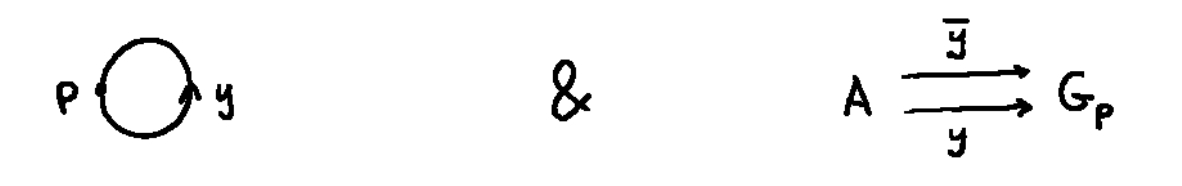
\includegraphics[width=0.5\linewidth]{sections/alicja/HNN loop and monomorphisms.jpeg}
    \caption{Graph $Y$ and monomorphisms it comes with}
    \label{loopHNN}
\end{figure}

\begin{importantexample}[\ref{HNN graph} for BS groups] \label{BS graph} In this example we will use multiplicative notation when talking about $\Z = \langle b \rangle$. 

We let $Y$ be a graph with vertex group $G_p = \Z$, and edge group $G_y = m\Z$. We set the monomorphism $a \mapsto a^y$ to be $(b^m)^k \mapsto (b^m)^k$, and this identifies $m\Z$ with its copy living inside $\Z$. We let the other morphism be $\phi: m\Z \to \Z$, $(b^m)^k \mapsto (b^n)^k$. Note, that $\phi$ is actually mapping $m\Z$ into $n\Z$ inside $\Z$. Using that observation, the fundamental group of $Y$ is $\Z \ast _\phi$, which by \ref{BS as HNN} is the group $BS(m,n)$. Finally, note that $g_y$ mentioned in \ref{HNN graph} is equal to $t$ in this case.
\end{importantexample}

The next construction will be based on \cite[pages 23-24]{GoPaXi24}, cross-referenced with \cite{Wil} and \cite{BajoHNN}, where in the latter the less general case is discussed.

\begin{construction} \label{universalcover}
    Let $\mathbb{X} = (G,\Gamma)$ be a graph of groups, with underlying graph $\Gamma$ and fundamental group $\pi = \pi_1(G,\Gamma,T)$, where $T$ is a maximal tree of $\Gamma$.
    The Bass-Serre tree $\Tilde{X}$ of $\mathbb{X}$ is constructed as follows:
    \begin{itemize}
        \item it has vertices $vert \: \Tilde{X} = \{\pi/G_x\:|\: x \in vert\:\Gamma\}$, and
        \item its edges are $edge \: \Tilde{X}_+ = \{\pi/\phi(G_y) \: | \: y \in edge \:\Gamma_+ \}$, where
        \item for each $g\phi(G_y) \in edge \: \Tilde{X}_+$, $o(g\phi(G_y)) = gG_{o(y)}$ and $t(g\phi(G_y)) = gg_yG_{t(y)}$.
    \end{itemize}
\end{construction}

Having stated the construction, two questions should come to mind, namely - why is this a connected graph and moreover, a tree. Instead of addressing those, we will see what this construction gives for $BS(m,n)$, and hopefully believe the resulting graph is indeed a tree.


\begin{importantexample}
    To construct the Bass-Serre tree of the Baumslag-Solitar group $BS(m,n) = \langle b,t \: | \: tb^mt^{-1} = b^n \rangle$, we will use its graph of groups $\mathbb{X}$, which was described in \ref{BS graph}. Recall that $\mathbb{X}$ is a loop, i.e. has only one vertex, with vertex group $G_x = \Z = \langle b\rangle$, and an edge attached to said vertex, with edge group $G_y = m\Z$. Thus, vertices of $\Tilde{X}$ are cosets $g\Z$, and edges are $g(\phi(m\Z)) = g(n\Z)$, with $g \in BS(m,n)$. Let us denote $H=n\Z$. Finally, for each edge $gH$, if we assume it is in $edge \: \Tilde{X}_+$, $o(gH) = g\Z$ and $t(gH) = gt(n\Z)$.
    The resulting graph is depicted in \ref{BS tree}.
    The following are worth noting:
    \begin{enumerate}
        \item because of the relation $tb^mt^{-1} = b^n$, we get that $tb^m = b^nt$ and $b^mt^{-1} = t^{-1}b^n$. Thus $b^nt\Z = tb^m\Z = t\Z$ are all the same coset, and if $0 \le f <n$, then $b^ft\Z \neq t\Z$. This is because, if they were equal, it would mean that we have a relation $b^f = tb^lt^{-1}$ for some $l \in \Z$, which is not true. Similarly, $b^mt^{-1}\Z = t^{-1}b^n\Z = t^{-1}\Z$ and for all $0 \le f <m$, then $b^ft^{-1}\Z \neq t^{-1}\Z$.
        This explains why the described vertices appear as adjacent to the vertex labelled by $\Z$ in the figure.
        \item As $BS(m,n)$ acts on $\Tilde{X}$ by automorphisms, and above we saw that the coset $\Z$ corresponds to a vertex of valence $n+m$, all vertices will have that valence. 
    \end{enumerate}
\end{importantexample}

\begin{figure}[ht]
    \centering
    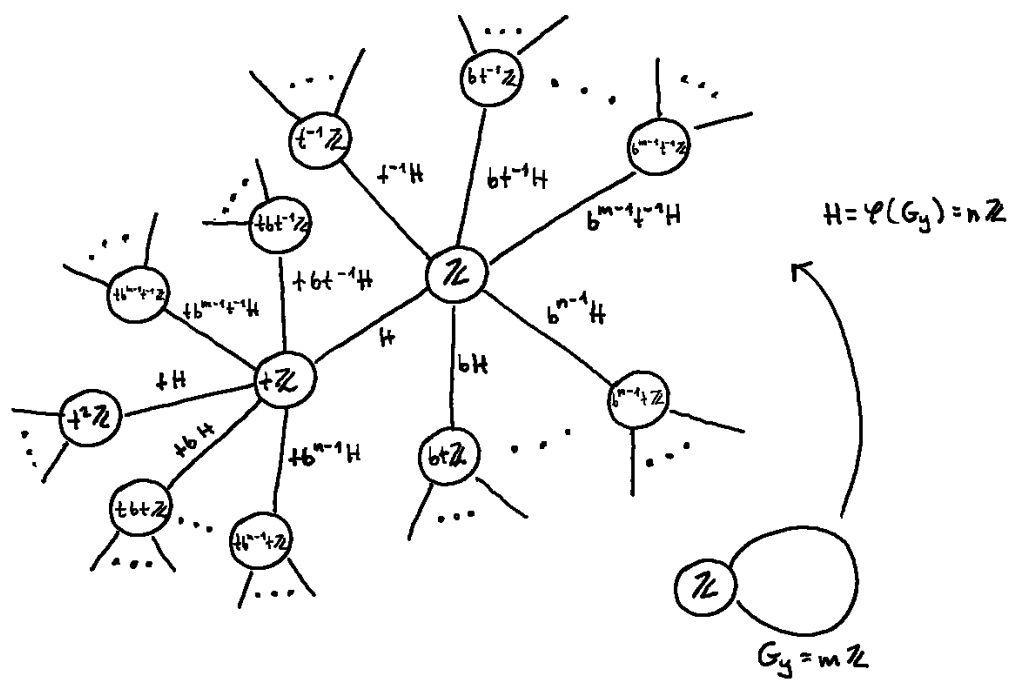
\includegraphics[scale = 0.38]{sections/alicja/Tree of BS(m,n) corrected.jpeg}
    \caption{Bass-Serre tree for $BS(m,n)$}
    \label{BS tree}
\end{figure}

We have discussed the graph with fundamental group $BS(m,n)$, as well as, the tree associated to it. We can now go on to generalise Baumslag-Solitar groups.

\subsection{Generalised Baumslag-Solitar (GBS) groups}

In the previous section we saw the connections certain trees and graphs of groups. It should then come as no surprise that we can define our group in terms of one or the other. Depending on what properties of $GBS$ groups one wants to explore, one of the following definitions might be preferable.

\begin{definition}\cite{For03}
    A \emph{generalised Baumslag-Solitar tree} is a $G$-tree whose vertex and edge stabilisers are all infinite cyclic. The groups $G$ that arise this way are called \emph{generalised Baumslag-Solitar groups}.
\end{definition}

\begin{definition}\cite{Le07}\label{GBSgofg}
    A \emph{generalised Baumslag-Solitar group} $G$ is the fundamental group of a graph of groups $\Gamma$ whose vertex and edge groups are all infinite cyclic.
\end{definition}

Let us start by looking at some examples of $GBS$ groups.

\begin{example}
    As one would hope, Baumslag-Solitar groups $BS(m,n)$ are $GBS$ groups. One can see it using the definition \ref{GBSgofg} -  a graph with the fundamental group $BS(m,n)$ which we obtained in \ref{BS graph} has vertex and edge groups $\Z$ and $m\Z$, respectively.
\end{example}

\begin{example} 
    A torus knot group, $T(p,q) = \langle x,y | x^p = y^q \rangle$ where $p$,$q$ are distinct primes, is a $GBS$ group.

    This can be seen by considering the graph of groups from figure \ref{T(p,q) graph}, which by the discussion in \cite{Jo23} has $T(p,q)$ as its fundamental group.
\end{example}

\begin{figure}[h]
    \centering
    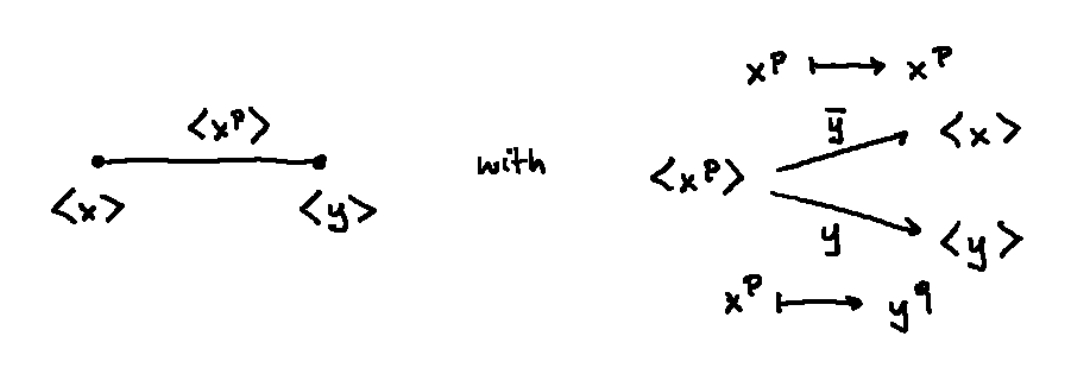
\includegraphics[width=0.5\linewidth]{sections/alicja/Graph for T(p,q).jpeg}
    \caption{Graph of groups for $\langle x \rangle \ast_{x^p = y^q} \langle y \rangle$ and morphisms it comes with} 
    \label{T(p,q) graph}
\end{figure}

Having seen the two examples which get quoted most often in the literature as first examples of $GBS$ groups, we can now consider a collection of results about this class of groups.

\subsubsection{Elementary $GBS$ groups}
Firstly, note that, as $GBS$ graphs $\Gamma$ have all edge and vertex groups infinite cyclic, we can choose their generators. Then, the inclusion maps of edge groups into vertex groups become multiplications by non-zero integers. Thus, we can endow an oriented edge $e$ with a label $\lambda_e \in \Z \setminus \{0\}$ describing the inclusion of $G_e$ into $G_{o(e)}$. A pair of opposite edges $\epsilon = (e,\overline{e})$ is a non-oriented edge, and it can be endowed with a label $(\lambda_e,\lambda_{\overline{e}})$. Note, that this construction can be applied to both loops and segments of a graph $\Gamma$.

In \cite{Le07} Levitt makes the following distinction.

\begin{remark} \label{elemlinegbs}
    The elementary $GBS$ groups $G$, with $\Gamma$ being a graph of groups with $\pi_1(\Gamma) = G$ are:
    \begin{itemize}
        \item $\Z$ with $\Gamma$ = point,
        \item $\Z^2$ with $\Gamma$ = $(1,1)$-loop,
        \item Klein bottle group $\langle x,t \: | \: txt^{-1} = x^{-1} \rangle = \langle a,b \: | \: a^2 = b^2\rangle$ with either $\Gamma$ = $(1,-1)$-loop or $(2,2)$-segment.
    \end{itemize}
    The feature that the above have in common is that the Bass-Serre tree $T$ associated to each of them is either a point or a line. Moreover, they are the only graphs for which that holds.
\end{remark}

\begin{figure}[h]
    \centering
    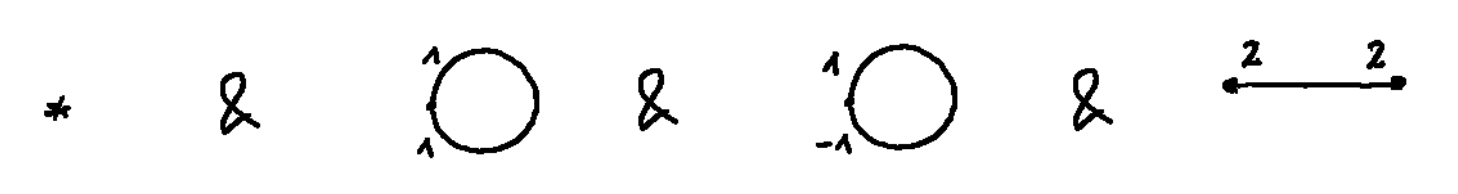
\includegraphics[scale = 0.15]{sections/alicja/Elementary graphs.jpeg}
    \caption{Graphs with elementary $GBS$ fundamental groups}
    \label{elementarygraphs}
\end{figure}

\subsubsection{Properties of $GBS$ groups developed in \cite{For03}} This paper concerns JSJ decompositions and their uniqueness for finitely presented groups, and uses $GBS$ trees as examples. Thus, the paper reviews some properties of $GBS$ groups.

Firstly, we will state some definitions for the situation when we have any $G$-tree.
\begin{definition}
    Let $T$ be a $G$-tree. An element $\gamma \in G$ is called \emph{elliptic} if it fixes a vertex of $T$. Otherwise $\gamma$ is said to be \emph{hyperbolic}.
    
    Elements $\gamma,\delta \in G$ are defined to be \emph{commensurable} if there exist $m,n \in \Z\setminus \{0\}$ such that $\gamma^m = \delta^n$. The \emph{commensurator} of $\gamma$ is the set of all $\delta \in G$ such that $\delta\gamma\delta^{-1}$ and $\gamma$ are commensurable. We denote it as $Comm(\gamma)$.
\end{definition}

\begin{remark}
    As shown in \cite[Proposition 24]{Ser80} if $\gamma$ is hyperbolic, then there is a $\gamma$-invariant path (or line) in $T$, on which $\gamma$ acts by translation. We call this path an \emph{axis} of $\gamma$.
\end{remark}

\begin{lemma} (\cite[2.5]{For03}, \cite[2.1]{Le07} combined)
    Let $T$ be a $G$-tree. If $\gamma \in G$ is hyperbolic then $Comm(\gamma)$ stabilises its axis. If additionally $T$ is a $GBS$ tree with $G$ non-elementary, then any two nontrivial elliptic elements $\gamma,\delta$ are commensurable, and the commensurator for an elliptic element $\gamma$ is the whole of $G$.
\end{lemma}

\begin{remark}
    Assuming that $T$ is a $GBS$ tree with non-elementary $G$ actually grants us something more. According to \cite[2.1]{Le07}, in that situation, an element $\gamma \in G$ is elliptic if and only if its commensurator equals $G$. This is because, if $\gamma$ is hyperbolic, then its axis is invariant under $Comm(\gamma)$. Thus, $G \neq Comm(\gamma)$, as $T$ is not a point or a line. The latter comes from the feature that we pointed out about the graphs of elementary groups in \ref{elemlinegbs}.
\end{remark}

We are also able to state some properties of $G$, provided its a $GBS$ group.

\begin{lemma}
    Let $T$ be a $GBS$ tree with group $G \ncong \Z$. Then:
    \begin{enumerate}
        \item G is not free;
        \item G is torsion free and has cohomological dimension 2;
        \item G has one end, if it is finitely generated;
        \item T contains a $G$-invariant line if and only if $G$ is isomorphic to $\Z \times \Z$ or the Klein bottle group.
    \end{enumerate}
    \textcolor{red}{I am not sure if I want to dive into cohomological dimension, I guess I could reference the reader to Talia's section for ends}
\end{lemma}

\textcolor{red}{currently writing this}

\subsubsection{Classification of $GBS$ graphs}

\begin{remark}
    Note, that sometimes $GBS$ graphs are called \emph{graphs of $\Z$s}. This again points at how $GBS$ groups generalise Baumslag-Solitar groups, as $BS$ groups are precisely the HNN extensions of $\Z$.
\end{remark}

The following theorem of Whyte classifies graphs of $\Z$, thus by the above remark, $GBS$ graphs.

\begin{theorem}\cite[Theorem 0.1]{WH01}\label{classgrZ}
    If $\Gamma$ is a graph of $\Z$s and $G= \pi_1(\Gamma)$ then exactly one of the following is true:
    \begin{enumerate}
        \item $G$ contains a subgroup of finite index of the form $F_n \times \Z$, where $F_n$ is the free group on $n$ generators.
        \item $G = BS(1,n)$ for some $n > 1$.
        \item $G$ is quasi-isometric to $BS(2,3)$.
    \end{enumerate}
\end{theorem}

\begin{corollary}
    All the groups $BS(m,n)$ with $1 < m <n$ are quasi-isometric to each other.
\end{corollary}

\begin{remark}
    Recall that a map $f: X \to Y$ between two metric spaces is called a quasi-isometry if there exist constants $\lambda \ge 1$, $c \ge 0$ and $K$ such that:
    \begin{enumerate}
        \item $\frac{1}{\lambda}d_X(x,x') - c \le d_Y(f(x),f(x')) \le \lambda d_X(x,x') + c$ (q-i embedding), and
        \item $\forall y \in Y$ $ \exists x \in X$ with $d(y,f(x)) \le K$ (quasi-surjectivity).
    \end{enumerate}
    We can think of a finitely generated group $G$ as a metric space, as given a generating set $S$ of $G$, we can consider the word metric $d_S$. Recall, that $d_S(g,h) = l_S(g^{-1}h) = \{length \; of \; a\;shortest \; word \; representing \; g^{-1}h \; in \; S\cup S^{-1} \}$. It is a fact that if $S$, $T$ are both finite generating sets for $G$, then $(G,d_S)$ and $(G,d_T)$ are quasi-isometric. We say that two finitely generated groups $G$, $H$ are \emph{quasi-isometric} if there exists a quasi-isometry $f: (G,d_S) \to (H,d_T)$ where $S$, $T$ are generating sets of $G$, $H$, respectively.
\end{remark}

In the sketch below we will be following an outline that was provided in \cite{WH01}.

\begin{proof}[Idea of proof of \ref{classgrZ}]
    Let us start by letting $G$ be the fundamental group of a graph of groups $\Gamma$, $T$ a Bass-Serre tree for $G$. The main ideas of the argument are:
    \begin{itemize}
        \item We can construct $X_G$ which in appropriate sense reflects the geometry of $G$, and on which $G$ acts nicely.
        \item The constructed $X_G$ is a contractible $2$-complex, which topologically is a product $T \times \R$. Metrically, it differs from the product metric by $v \times \R$ getting scaled by a fitting warping function $T \to \R^+$.
        \item Due to the construction, the warping function depends on height change between vertices. Said height change can be seen as quantitative analogue of orientation.
        \item The classification of graphs of $\Z$s reduces to classifying coarsely oriented trees. This is by showing that being given a quasi-isometry between the graphs there is a quasi-isoetry coarsely respecting orientation between trees, and vice versa when given a coarsely orientation preserving quasi-isometry between Bass-Serre trees.
        \item Due to caring about coarsely orientation preserving quasi-isometries, we can consider a special type of trees and develop their classification.
        \item The final quasi-isometries are by considering lines of "constant slope" and building quasi-isometries line by line
    \end{itemize}
The above are sufficient to classify graphs of $\Z$s up to quasi-isometry.
\end{proof}




